\documentclass[12pt,a4paper]{article}

% -------------------- PAKETI --------------------
\usepackage[utf8]{inputenc}
\usepackage[serbian]{babel}
\usepackage{amsmath}
\usepackage{graphicx}
\usepackage{geometry}
\usepackage{setspace}
\usepackage{hyperref}
\usepackage{tocloft}
\usepackage{float}
\usepackage{array}
\usepackage{ragged2e}
\renewcommand{\arraystretch}{1.2}

\renewcommand{\cftsecleader}{\cftdotfill{\cftdotsep}}
\renewcommand{\cftsubsecleader}{\cftdotfill{\cftdotsep}}

\geometry{margin=2.5cm}
\onehalfspacing

% -------------------- NASLOV --------------------
\title{Monotasking vs Multitasking}
\author{Miloš Biočanin 107/2020}
\date{Jun 2026}

\begin{document}

% -------------------- NASLOVNA STRANA --------------------
\maketitle
\thispagestyle{empty}
\newpage

% -------------------- SADRŽAJ --------------------
\pagenumbering{arabic}
\tableofcontents
\newpage

% -------------------- UVOD --------------------
\section{Uvod}

U savremenom društvu postoji sve veći pritisak na pojedince da svoje vreme koriste što efikasnije. Kako se ljudi svakodnevno suočavaju sa sve većim brojem obaveza, kao i težnjom ka postizanju što većeg broja ciljeva u ograničenom vremenskom periodu, od njih se često očekuje da obavljaju više aktivnosti istovremeno. Dodatni uticaj na ovakav način rada ima ubrzan razvoj informacionih tehnologija i široka dostupnost interneta i mobilnih uređaja.

Pametni telefoni omogućili su neprekidan pristup informacijama, elektronskoj pošti, društvenim mrežama i različitim komunikacionim kanalima, čime su granice između rada, učenja i slobodnog vremena postale znatno manje izražene.

Kao posledica ovih promena, multitasking je postao sastavni deo svakodnevnog života velikog broja ljudi. Mogućnost istovremenog obavljanja više aktivnosti često se posmatra kao pokazatelj produktivnosti i efikasnog upravljanja vremenom. Međutim, postavlja se pitanje da li multitasking zaista doprinosi boljoj efikasnosti ili dovodi do smanjenja koncentracije i kvaliteta izvršavanja zadataka, dok samo pruža osećaj veće produktivnosti. Sve je više dokaza da ovakav način rada ne mora nužno dovesti do boljih rezultata.

Sa druge strane, sve više pažnje posvećuje se konceptu monotaskinga, odnosno fokusiranju na jedan zadatak u određenom vremenskom periodu. Brojna istraživanja ukazuju na to da često prebacivanje pažnje između različitih aktivnosti može negativno uticati na koncentraciju, kvalitet rada i sposobnost pamćenja \cite{watson2010, ophir2009}.

Tema monotaskinga i multitaskinga posebno je značajna među studentima i zaposlenima, jer način organizacije pažnje direktno utiče na rezultate učenja, obavljanje poslovnih zadataka i svakodnevno funkcionisanje. Razumevanje načina na koji ljudski mozak obrađuje informacije može pomoći u razvijanju efikasnijih radnih i obrazovnih navika.

Cilj ovog rada jeste analiza razlika između monotaskinga i multitaskinga, kao i njihovog uticaja na produktivnost, koncentraciju i kvalitet izvršavanja zadataka. U radu će biti predstavljene osnovne karakteristike oba pristupa, prednosti i mane, kao i rezultati određenih istraživanja iz ove oblasti.

U radu će najpre biti definisani osnovni pojmovi monotaskinga i multitaskinga, nakon čega će biti razmotrene njihove prednosti i nedostaci, kao i njihov uticaj na studente i svakodnevni rad.


% -------------------- GLAVNI DEO --------------------

\section{Multitasking}

\subsection{Multitasking – pojam i karakteristike}

Multitasking predstavlja način obavljanja više aktivnosti u istom vremenskom periodu, pri čemu pojedinac pokušava da istovremeno izvršava više zadataka ili da ih kombinuje u kratkim vremenskim intervalima \cite{APA}. U savremenom okruženju, ovaj pojam se najčešće povezuje sa korišćenjem digitalnih tehnologija, gde ljudi istovremeno komuniciraju putem poruka, koriste društvene mreže, prate sadržaje na internetu i obavljaju radne ili obrazovne obaveze.

Na prvi pogled, multitasking deluje kao efikasan način organizacije vremena koji omogućava da se u kratkom periodu završi veći broj zadataka. Zbog stalne dostupnosti informacija i komunikacionih kanala, posebno putem pametnih telefona, ovaj način rada postao je deo svakodnevnog života velikog broja ljudi.

Međutim, važno je napraviti razliku između stvarnog istovremenog obavljanja više zadataka i fenomena poznatog kao \textit{task switching}, odnosno brzog prebacivanja pažnje između različitih aktivnosti. Istraživanja iz oblasti kognitivne psihologije pokazuju da ljudski mozak ima ograničene kapacitete za paralelnu obradu složenih informacija, zbog čega se većina oblika multitaskinga u praksi svodi na konstantno preusmeravanje pažnje.


\subsection{\textit{Task switching} i kognitivni troškovi}

Pojam \textit{task switching} označava proces prebacivanja pažnje sa jednog zadatka na drugi. Umesto stvarnog istovremenog obavljanja više aktivnosti, ljudski mozak zapravo konstantno menja fokus između različitih zadataka, što zahteva dodatne kognitivne resurse \cite{rubinstein2001}.

Istraživanja koja su sproveli Rubinstein i saradnici pokazala su da ovakvo prebacivanje između zadataka dovodi do tzv. \textit{switching cost}, odnosno gubitka vremena i smanjenja efikasnosti \cite{rubinstein2001}. Svaki put kada osoba prekine jednu aktivnost i pređe na drugu, potrebno je određeno vreme da se ponovo uspostavi fokus, razume kontekst i prilagodi novim zahtevima.

Ovi kratki, ali ponavljajući prekidi mogu se akumulirati i dovesti do značajnog pada ukupne produktivnosti, povećanja broja grešaka i većeg mentalnog zamora. Iako multitasking može delovati kao efikasan način rada, u praksi on često predstavlja niz brzih prekida pažnje koji utiču na kvalitet izvršavanja složenih zadataka.

Takođe, fenomen poznat kao \textit{attention residue} (ostatak pažnje) ukazuje na to da nakon prelaska sa jednog zadatka na drugi deo pažnje ostaje “vezan” za prethodnu aktivnost, što dovodi do smanjenja kognitivne efikasnosti na novom zadatku \cite{leroy2009}.

\subsection{Uticaj multitaskinga na pažnju i kognitivnu kontrolu}

Kognitivna kontrola predstavlja skup mentalnih procesa koji omogućavaju usmeravanje i regulisanje mišljenja i ponašanja u skladu sa ciljevima, posebno u situacijama kada postoji više konkurentnih informacija ili zadataka. Ona uključuje sposobnosti kao što su održavanje pažnje na relevantnom zadatku, inhibicija distrakcija, prebacivanje između zadataka i ažuriranje radne memorije.

Istraživanje koje su sproveli Ophir i saradnici ispitivalo je razlike između osoba koje često istovremeno koriste više medija (engl. \textit{heavy media multitaskers}) i osoba koje to čine ređe (engl. \textit{light media multitaskers}). Rezultati istraživanja pokazali su da osobe sklone čestom media multitaskingu imaju veće poteškoće u filtriranju nevažnih informacija iz okruženja i teže održavaju pažnju na relevantnim zadacima \cite{ophir2009}.

Pored toga, utvrđeno je da osobe koje često praktikuju media multitasking imaju slabiju sposobnost ignorisanja nebitnih informacija koje su već uskladištene u memoriji, kao i manju efikasnost pri prebacivanju između različitih zadataka. Ovi rezultati ukazuju na to da česta istovremena upotreba više medija može biti povezana sa promenama u načinu na koji pojedinci upravljaju pažnjom i kognitivnom kontrolom.

Autori pretpostavljaju da osobe sklone intenzivnom media multitaskingu imaju izraženiju tendenciju ka obraćanju pažnje na spoljašnje stimuluse, zbog čega češće reaguju na distrakcije iz okruženja. Nasuprot tome, osobe koje ređe praktikuju multitasking pokazuju veću sposobnost usmeravanja i održavanja pažnje na jednom zadatku uprkos prisustvu ometajućih faktora \cite{ophir2009}.

\subsection{Uticaj multitaskinga na mozak}

Loh i Kanai su utvrdili da osobe sa višim nivoom media multitaskinga imaju manju gustinu sive mase u anteriornom cingularnom korteksu (ACC), regionu mozga koji je povezan sa kognitivnom kontrolom, donošenjem odluka i održavanjem pažnje (Slika \ref{fig:lohkanai}). Ovaj nalaz sugeriše da intenzivno korišćenje više medija istovremeno može biti povezano sa promenama u moždanim strukturama odgovornim za kontrolu pažnje \cite{loh2014}.

Anteriorni cingularni korteks (ACC) igra ključnu ulogu u kognitivnoj kontroli, održavanju pažnje i inhibiciji distrakcija. Zbog toga se promene u strukturi ovog regiona mogu povezati sa razlikama u efikasnosti upravljanja pažnjom i obradom konkurentnih informacija \cite{devinsky1995}.

\begin{figure}[h]
    \centering
    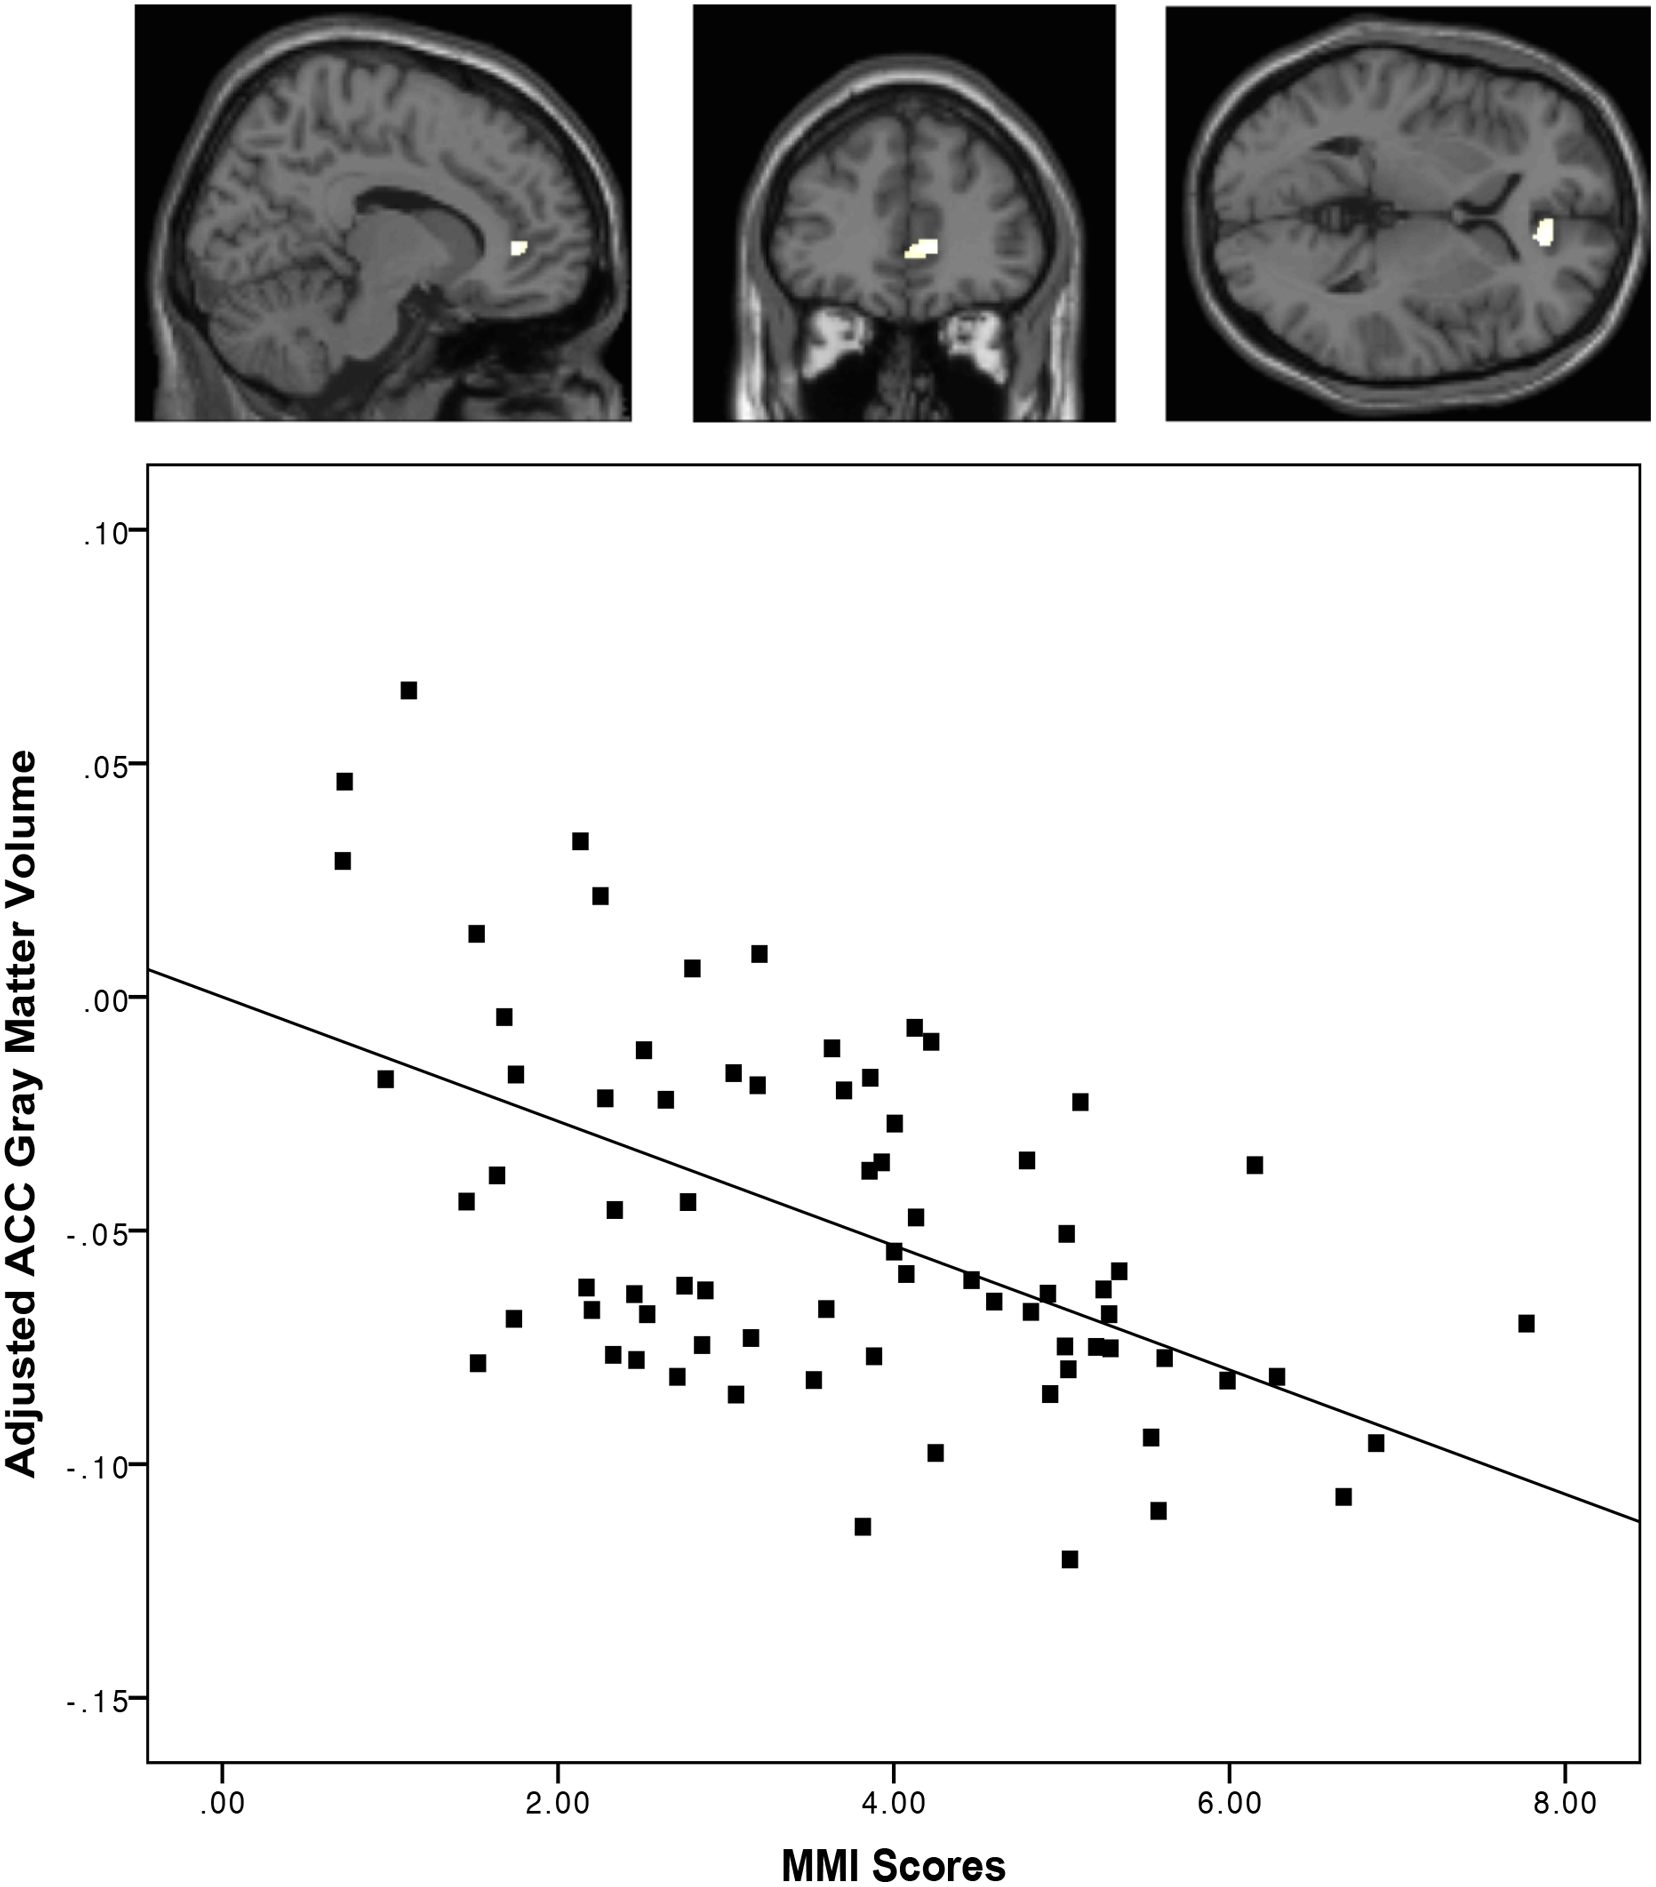
\includegraphics[width=0.75\textwidth]{grey-matter-volume.png}
    \caption{Korelacija između gustine sive mase u ACC i media multitaskinga}
    \label{fig:lohkanai}
\end{figure}

\subsection{\textit{Supertaskers}}

Iako većina istraživanja ukazuje na negativne efekte čestog prebacivanja pažnje između zadataka, postoje i pojedinci koji pokazuju izuzetne sposobnosti u ovom domenu. Takozvani “supertaskeri” predstavljaju mali procenat populacije koji je u stanju da obavlja više zadataka istovremeno bez značajnog pada u performansama. Međutim, istraživanja pokazuju da je ovakva sposobnost veoma retka i da ne predstavlja tipičan obrazac ponašanja u opštoj populaciji \cite{watson2010}.

% -------------------- MONOTASKING --------------------

\section{Monotasking}

\subsection{Monotasking - pojam i karakteristike}

Monotasking predstavlja pristup radu i učenju koji se zasniva na usmeravanju pažnje na jedan zadatak u određenom vremenskom periodu, bez istovremenog obavljanja ili preplitanja sa drugim aktivnostima. Za razliku od multitaskinga, koji podrazumeva česte promene fokusa, monotasking se fokusira na održavanje kontinuirane pažnje i minimizovanje prekida tokom izvršavanja zadatka.

Osnovna ideja monotaskinga jeste da ljudski mozak postiže bolje rezultate kada je kognitivni kapacitet usmeren na jednu aktivnost, jer se na taj način smanjuje opterećenje radne memorije i povećava efikasnost obrade informacija. Ovaj pristup je posebno značajan kod složenih zadataka koji zahtevaju duboko razumevanje, analizu i dugotrajnu koncentraciju

% -------------------- POREĐENJE --------------------

\section{Poređenje monotaskinga i multitaskinga}

Iako se multitasking u savremenom društvu često povezuje sa većom produktivnošću, brojna istraživanja ukazuju da često prebacivanje pažnje između zadataka može dovesti do povećanog kognitivnog opterećenja i smanjenja efikasnosti \cite{ophir2009, rubinstein2001}. 

Nasuprot tome, monotasking omogućava kontinuirano usmeravanje pažnje na jedan zadatak, čime se smanjuju kognitivni troškovi povezani sa prebacivanjem između aktivnosti.

Tabela \ref{tab:poredjenje} prikazuje najvažnije razlike između monotaskinga i multitaskinga.

\begin{table}[H]
\centering
\caption{Poređenje monotaskinga i multitaskinga}
\label{tab:poredjenje}

\begin{tabular}{|
>{\RaggedRight\arraybackslash}p{3.8cm}|
>{\RaggedRight\arraybackslash}p{5cm}|
>{\RaggedRight\arraybackslash}p{5cm}|}
\hline

\textbf{Karakteristika} & \textbf{Monotasking} & \textbf{Multitasking} \\
\hline

Upravljanje pažnjom & Fokus je usmeren na jedan zadatak tokom dužeg vremenskog perioda. & Pažnja se često prebacuje između više zadataka ili izvora informacija. \\
\hline

Kognitivno opterećenje & Manje kognitivno opterećenje usled odsustva čestog preusmeravanja pažnje. & Povećano kognitivno opterećenje zbog učestalog \textit{task switching}-a. \\
\hline

Kvalitet izvršavanja zadataka & Omogućava dublju obradu informacija i manji broj grešaka. & Može dovesti do površnije obrade informacija i većeg broja grešaka. \\
\hline

Pamćenje i učenje & Pogodniji za usvajanje složenih informacija i dugoročno pamćenje. & Česti prekidi pažnje mogu negativno uticati na procese učenja i pamćenja. \\
\hline

Pogodne situacije za primenu & Složeni zadaci koji zahtevaju visok nivo koncentracije i kreativnosti. & Jednostavne ili rutinske aktivnosti koje ne zahtevaju značajne kognitivne resurse. \\
\hline

\end{tabular}
\end{table}

Monotasking se pokazuje kao efikasniji pristup u situacijama koje zahtevaju kontinuiranu koncentraciju, rešavanje složenih problema i obradu većeg broja informacija. Odsustvo čestih prekida omogućava stabilniji tok razmišljanja i kvalitetnije izvršavanje zadataka \cite{rubinstein2001,leroy2009}.

Sa druge strane, određeni oblici multitaskinga mogu biti korisni kada je potrebno obavljati više jednostavnih ili visoko automatizovanih aktivnosti istovremeno. Pored toga, pojedina savremena radna okruženja zahtevaju upravljanje većim brojem informacionih tokova i komunikacionih kanala, zbog čega potpuno izbegavanje multitaskinga često nije moguće.

Ipak, rezultati većine istraživanja ukazuju da se kod kognitivno zahtevnih aktivnosti monotasking pokazuje kao efikasniji pristup, prvenstveno zbog smanjenja kognitivnih troškova povezanih sa prebacivanjem pažnje i boljeg održavanja fokusa \cite{ophir2009, rubinstein2001}.

% ------------- STRATEGIJA ZA UMANJENJE -------------

\section{Metodološki pristupi povećanju koncentracije i smanjenju distrakcija}

Pristupi unapređenju koncentracije u uslovima čestih prekida pažnje zasnivaju se na nalazima koji ukazuju da multitasking dovodi do povećanog kognitivnog opterećenja i potrebe za periodima oporavka pažnje \cite{schumann2022}. Na osnovu ovih nalaza, u literaturi se izdvajaju tri osnovna metodološka pravca: kontrola okruženja, strukturalno upravljanje vremenom i regulacija kognitivne pažnje.

Prvi pristup odnosi se na minimizaciju spoljašnjih izvora distrakcije. Eksperimentalna istraživanja pokazuju da prisustvo obaveštenja, digitalnih prekida i konkurentnih stimulusa značajno povećava učestalost preusmeravanja pažnje, što direktno utiče na smanjenje performansi u kognitivno zahtevnim zadacima. Zbog toga se kao metodološki princip koristi redukcija stimulusa koji iniciraju \textit{task switching} procese.

Drugi pristup zasniva se na vremenskoj segmentaciji rada, pri čemu se aktivnosti organizuju u jasno definisane intervale usmerene na jedan zadatak. Ovakav metod, poznat kao \textit{time blocking}, smanjuje potrebu za čestim re-orijentisanjem pažnje i omogućava stabilnije održavanje radne memorije u okviru jednog zadatka.

Treći pristup odnosi se na kognitivnu regulaciju pažnje, odnosno sposobnost pojedinca da inhibira nerelevantne stimuluse i održi fokus na primarnom zadatku. Ovaj aspekt je povezan sa izvršnim funkcijama pažnje, koje omogućavaju selekciju relevantnih informacija i suzbijanje distrakcija tokom izvršavanja zadataka.

U okviru ovih pristupa, posebno se ističe važnost perioda oporavka pažnje, tokom kojih dolazi do smanjenja kognitivnog opterećenja i obnove sposobnosti održavanja fokusa. Ovi periodi se u literaturi posmatraju kao neophodan deo ciklusa rada, a ne kao pasivni prekid aktivnosti, što dodatno naglašava značaj strukturalnog planiranja rada i pauza.

Sve navedene metode ukazuju na to da unapređenje koncentracije ne predstavlja isključivo individualnu sposobnost, već rezultat interakcije između organizacije okruženja, strukture rada i mehanizama kognitivne kontrole.

% -------------------- ZAKLJUČAK --------------------

\section{Zaključak}

Analiza multitaskinga i monotaskinga pokazuje da se veći deo svakodnevnih aktivnosti koje se percipiraju kao istovremeno obavljanje više zadataka u praksi zapravo svodi na brzo prebacivanje pažnje između različitih aktivnosti. Ovakav oblik rada povezan je sa kognitivnim troškovima, smanjenjem efikasnosti i povećanim opterećenjem izvršnih funkcija, što je potvrđeno u istraživanjima iz oblasti kognitivne psihologije.

Nasuprot tome, monotasking omogućava stabilnije usmeravanje pažnje na jedan zadatak, čime se smanjuju negativni efekti povezani sa čestim prebacivanjem fokusa. Literatura ukazuje da ovakav pristup pogoduje dubljoj obradi informacija, boljem pamćenju i kvalitetnijem izvršavanju složenih kognitivnih zadataka.

Neurokognitivna istraživanja dodatno ukazuju da su strukture uključene u kognitivnu kontrolu i regulaciju pažnje, poput anteriornog cingularnog korteksa, značajne za uspešno upravljanje konkurentnim informacijama i održavanje fokusa. Razlike u ovim mehanizmima mogu doprineti individualnim razlikama u sposobnosti upravljanja multitasking situacijama.

Iako multitasking može biti funkcionalan u situacijama koje uključuju jednostavne ili automatizovane aktivnosti, rezultati većine istraživanja ukazuju da za kompleksne zadatke monotasking predstavlja efikasniji pristup. U tom smislu, izbor između ova dva pristupa zavisi od prirode zadatka, ali i od kognitivnih zahteva koje on postavlja.

Sveukupno posmatrano, rezultati rada ukazuju na to da savremeno digitalno okruženje podstiče učestalu fragmentaciju pažnje, dok strukturisanje rada kroz principe monotaskinga može doprineti stabilnijem kognitivnom funkcionisanju i većoj efikasnosti u obradi informacija.

\newpage

% -------------------- LITERATURA --------------------

\begin{thebibliography}{9}

\bibitem{watson2010}
Watson JM, Strayer DL. Supertaskers: Profiles in extraordinary multitasking ability. Psychonomic Bulletin \& Review. 2010;17(4):479-485. doi:10.3758/PBR.17.4.479

\bibitem{ophir2009}
Ophir E, Nass C, Wagner AD. Cognitive control in media multitaskers. Proceedings of the National Academy of Sciences. 2009;106(37):15583-15587. doi:10.1073/pnas.0903620106

\bibitem{APA}
American Psychological Association. Multitasking: Switching cost.
[Pristupljeno: 19.06.2026.] Dostupno na: https://www.apa.org/topics/research/multitasking

\bibitem{rubinstein2001}
Rubinstein JS, Meyer DE, Evans JE. Executive Control of Cognitive Processes in Task Switching. Journal of Experimental Psychology: Human Perception and Performance. 2001;27(4):763-797. doi:10.1037/0096-1523.27.4.763

\bibitem{leroy2009}

Leroy S. Why is it so hard to do my work? The challenge of attention residue when switching between work tasks. Organizational Behavior and Human Decision Processes. 2009;109(2):168-181. doi:10.1016/j.obhdp.2009.04.002

\bibitem{loh2014}

Loh KK, Kanai R (2014) Higher Media Multi-Tasking Activity Is Associated with Smaller Gray-Matter Density in the Anterior Cingulate Cortex. PLoS ONE 9(9): e106698. https://doi.org/10.1371/journal.pone.0106698

\bibitem{devinsky1995}

Devinsky O, Morrell MJ, Vogt BA. Contributions of anterior cingulate cortex to behaviour. Brain. 1995;118(1):279-306. doi:10.1093/brain/118.1.27

\bibitem{schumann2022}

Schumann F, Steinborn MB, Kürten J, Cao L, Händel BF and Huestegge L (2022) Restoration of Attention by Rest in a Multitasking World: Theory, Methodology, and Empirical Evidence. Front. Psychol. 13:867978. doi: 10.3389/fpsyg.2022.867978

\end{thebibliography}

\end{document}